\section*{General description}


Figure 1 shows the graph expanded to such an extent that the goal state is possible.
Figure 2 shows the extracted solution highlighted.

\subsection*{Explanation for expanding}

Initially, we have to expand since $S_{\textsc{Initial}} \neq S_{\textsc{Goal}}$.
Once we have expanded to $S_1$, we have to expand again, as the mutex between \texttt{sprkLwn} and \texttt{mowLwn} causes a mutex between \texttt{wetLwn} and \texttt{shortLwn}. Having expanded to $S_2$, this mutex is gone, and there are no other mutexes among the propositions relevant to the goal state, meaning we have found a solution.

\subsection*{Actions representing a plan that solves the gardening problem}

\begin{enumerate}
    \item \texttt{wcanFlwrs}
    \item \texttt{MowLwn}
    \item \texttt{sprkLwn}
\end{enumerate}

\subsection*{How the list in section 3 was obtained}

The solution sequence in section 3 was obtained by performing the \textsc{Graphplan} algorithm until the goal-state is non-mutexed.

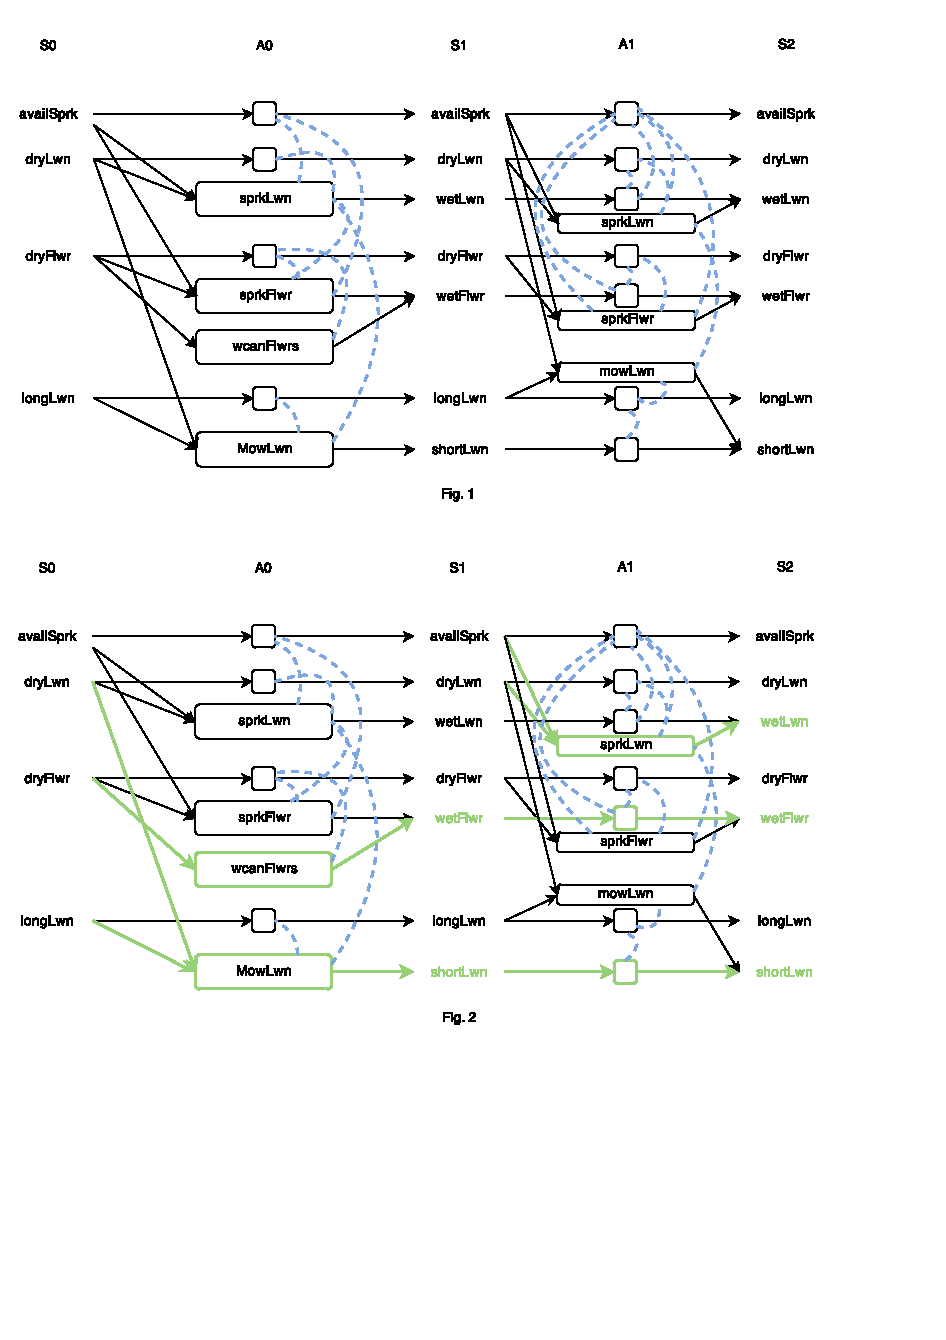
\includepdf[pages={1}]{../gardenplanning.pdf}
